\chapter{Techniques for Language Processing}
\label{chapt:NLP}
\section{Background}
Natural Language Processing is the application of computer science to study human languages using computers. Machine learning, a class of algorithms for predicting patterns in data, finds many applications in NLP. This section explores approaches to representing journal articles in a quantitative manner using NLP.
\section{Bag of Words}
A simple approach to representing a document is a \emph{bag of words} model. The document is split into component words in an unordered set. The model computes the number of distinct words in a corpus of documents, $N$. It then assigns each document in the corpus an $N$ dimensional vector $\mathbf{v}$. If document $A$ contains word $i$ 2 times, then $v_{A, i } = 2$. A simple example is given below:

Document A: \texttt{A good yield was obtained for a nucleophile}

Document B: \texttt{The nucleophile is a good donor}

Document C: \texttt{A gaussian basis was used}
\begin{table}[H]
\caption{Bag of words}
\label{tab:BAGOFWORDS}
\begin{center}
\begin{tabular}{||c|c|c|c||}
\hline
Vocabulary &  $\mathbf{v}_A$ & $\mathbf{v}_B$ & $\mathbf{v}_C$\\
\hline
A & 2 & 1 & 1\\
Good & 1 & 1 & 0\\
Nucleophile & 1 & 1 & 0 \\
Yield & 1 & 0 & 0\\
For & 1& 0 & 0\\
Is & 0 & 1 & 0\\
The & 1 & 0 & 0\\
Donor & 0 & 1 & 0\\
Was & 1 & 0 & 1\\
Gaussian & 0 & 0 & 1\\
Basis & 0 & 0 & 1\\
Used & 0 & 0 & 1\\
\hline
\end{tabular}
\end{center}
\end{table}
Table \ref{tab:BAGOFWORDS} shows vector representations for Documents A, B and C. The higher the scalar product of normalised $\mathbf{v}_A \cdot \mathbf{v}_A$, the more similar the documents are predicted to be:
 $$\mathbf{v}_A \cdot \mathbf{v}_A = 0.567 \ \ \ \ \mathbf{v}_A \cdot \mathbf{v}_C = 0.424 \ \ \ \ \mathbf{v}_B \cdot \mathbf{v}_C=0.200$$ 
and so documents A and B are the more similar.
The related \emph{bag of citations} model sets vector components according to the presence of citations. Both models are used by the scientific publishing industry\footnote{Dr. Colin Batchelor  (Senior Data Scientist, Royal Society of Chemistry), personal communication, February 2016},\footnote{P.E. Peter Murray-Rust, personal communication, February 2016}.
\section{Word2Vec}
\label{sec:WORD2VEC}
The \emph{Bag of Words} model treats words as atomic units, beneficial for robust computation. However, words have degrees of similarity to each other, which are not captured by bag of words models\cite{word2veckingqueen}. Distributed representations have been used to address this for some time\cite{distributedrepresentations}.

 A recent successful approach has been the Word2Vec algorithm\cite{word2vec1},\cite{word2vec2}.  Word2Vec uses a neural net to represent words as vectors in a continuous space. Vectors for words with similar meanings will point in similar directions in this `semantic space'. Word2Vec is fed a corpus sentence-by-sentence. The words within the sentences are semantically related, which the algorithm uses to infer word meanings. 
 
This is achieved with two architectures, Continuous Bag of Words (CBOW) and skipgram. The CBOW architecture uses a shallow neural net to predict a word's vector by summing or averaging the vectors of surrounding words in a training sentence. The skipgram architecture predicts the vectors of words surrounding the current training word. By training with many input sentences, prediction vectors are gradually improved. 

\begin{figure}[H]
    \centering
    \textbf{Word2Vec Training Architectures}\par\medskip
    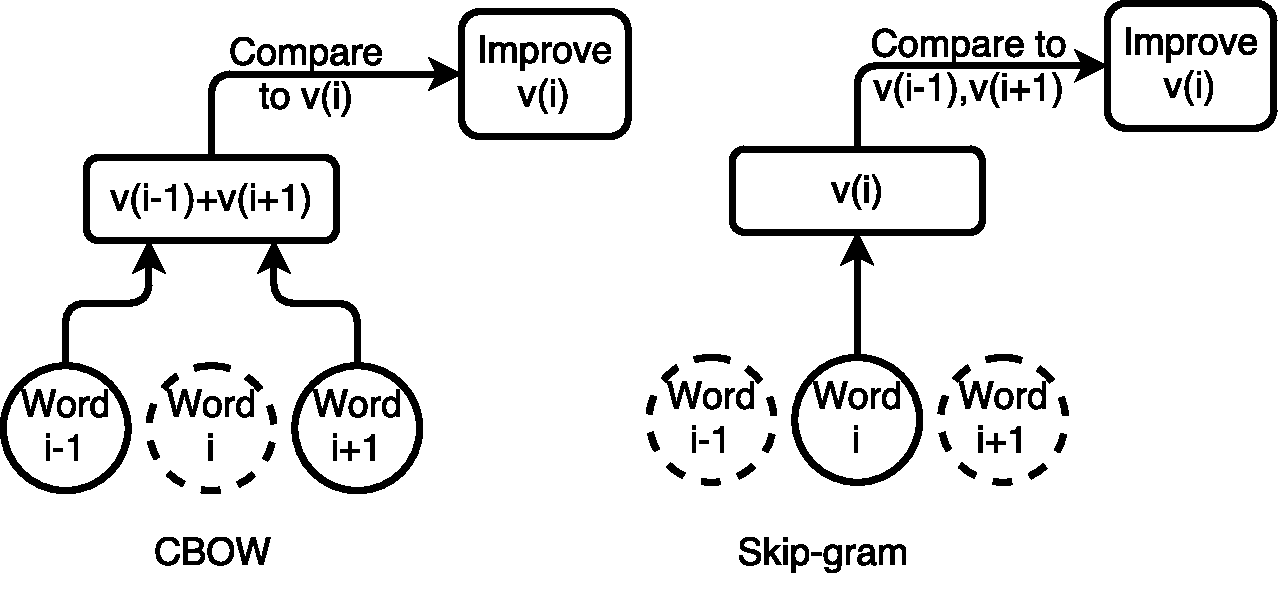
\includegraphics[width=\textwidth]{Natural_Language_Processing/cbow_v_skip.pdf}
    \caption[Word2Vec Training Architectures ]{The training architectures of the Word2Vec training algorithm. Word vectors are denoted $v(i)$ for word i. In CBOW word i is predicted by the vector found by summing vectors surrounding i, and $v(i)$ is adjusted to be closer to this prediction. In skipgram, word i's vector is pairwise compared to its context words (here i-1 and i+1 as a basis to improve $v(i)$). CBOW attempts to make words similar the sum of the surrounding words, skipgram attempts to minimise distance to each surrounding word.}
     \label{fig:CBOWSKIP}
\end{figure}

The training process is shown in figure \ref{fig:CBOWSKIP}. CBOW uses a fixed window of surrounding words. The order of words within the window does not matter, but because the window `slides' along as the algorithm considers words i+1, i+2... word ordering is represented in the model . In skipgram, a random number of surrounding words are used for the prediction vectors for word i. 

The model has added sophistication to reduce the importance of commonly occurring words, and to identify phrases. The word vectors that are produced encapsulate both semantic and syntactic meanings, and can be manipulated to represent concepts and relationships.
\begin{figure}[H]
    \centering
    \textbf{Word Vector Relationships}\par\medskip
    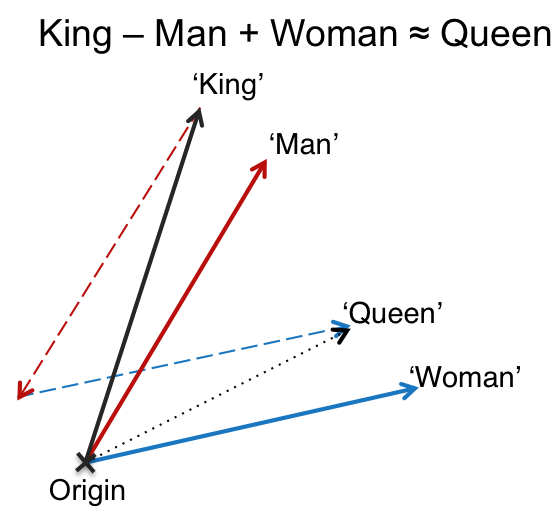
\includegraphics[height=6.5cm]{Natural_Language_Processing/KINGQUEEN.png}
    \caption[Word Vector Relationships]{Schematic Representation of how concepts can be represented in word vector space. Word2Vec is able to replicate this behaviour. The vector found by vec(‘King’)- vec(‘Man’)+vec(‘Woman’) is approximately equal to vec(‘Queen’). The model has been tested on thousands of similar examples\cite{word2vec2}\cite{word2veckingqueen}.}
     \label{fig:KINGQUEEN}
\end{figure}
Word2Vec models may represent concepts by vector algebraic operations on their word representations. Figure \ref{fig:KINGQUEEN} shows one famous example a Word2Vec model trained on the `Google News' text corpus was able to identify. \footnote{It is interesting to consider if chemical examples could be developed. This is considered further in \S\ref{chapt:RECOMMENDATIONS}.}

\section{Doc2Vec}
The Doc2Vec algorithm\cite{gensim} (an implementation of Paragraph Vectors\cite{doc2vec}) allows the Word2vec process to directly learn vectors representing documents. The CBOW architecture is adapted so that, in addition to word vectors, each document is associated with its own vector that contributes to predictions in training. The result is that documents can be represented by vectors in a document semantic space.

The nature of the collected meta-data detailed in \S\ref{chapt:DATA_ACQUISITION} (a large store of natural language) lends itself to the Word2Vec and Doc2Vec algorithms. The focus of the machine learning analysis phase of the project was directed at applying Word2Vec and Doc2Vec to $\Delta6$ to automatically learn and classify chemical semantic concepts.